\section{Intégration théorique}\label{sec:contrib:asteroid:theorie}
Dans cette section, nous présentons les fondements théoriques pour permettre l'intégration de supports persistants relationnels dans \textit{Astral}. Tout d'abord, nous présentons en détail les différents motifs d'évolution des données persistantes ou temps réel. Ceci est important car ces motifs ont des impacts sur le schéma de la base de donnée utilisé pour la persistance que nous présentons par la suite. Enfin, nous décrivons comment une relation persistante est représentée en tant que relation temporelle afin de pouvoir manipuler une base de donnée avec \textit{Astral}.

\subsection{Dynamique des données}
Nous nous intéressons à des systèmes où les données peuvent être persistantes ou sous forme de flux volatile. Nous remarquons aussi que les données évoluent suivant des motifs différents qui vont influencer la manière de les manipuler par la suite. Notamment, cela a un impact sur le schéma de la base de donnée relationnelle utilisée comme persistance.

Par définition, la persistance d'une donnée implique le stockage sur un support. Sa mise à jour sur ce support est une opération considérée comme lente\footnote{Cette lenteur a permit la création des SGFD à la fin des années 90.}. Ainsi, il est difficile de supposer possible l'utilisation d'un SGBD seul pour gérer toutes les données du système. Il est nécessaire de séparer les intérêts de chacun des systèmes. Les données du systèmes sont considérées en quatre dynamiques divisées en deux catégories : les meta-données et les volatiles. 

Tout d'abord, celles que nous qualifions de meta-données, rassemblés dans des catalogues (typiquement, des relations persistantes). Celles-ci sont décomposés en deux classes de dynamiques :
\begin{itemize}
	\item[\textbf{Statique}] correspond à des méta-données qui ne changent jamais par essence. Comme leur valeur est constante, leur utilisation en interrogation continue est similaire à une relation temporelle $R$ figée : $R^{t_0}$. Par exemple, le numéro de série d'un équipement est une information qui par nature est immuable.
	\item[\textbf{Stable}] correspond à des méta-données considérées la plupart du temps comme figée. Elles ne sont toutefois pas immuable et peuvent subir des modifications. Bien que leur utilisation soit avant tout une interrogation instantanée, en interrogation continue elles sont manipulable par une relation temporelle $R$ sans manipulation temporelle. Par exemple, un paramètre de configuration d'un équipement du réseau local est considéré comme stable.
\end{itemize}

La deuxième catégorie rassemble les données volatiles évoluant en temps réel. Elles prennent la forme de flux de données et peuvent posséder deux dynamiques :
\begin{itemize}
	\item[\textbf{Périodique}] rassemble les données dont l'historique forme un flux régulier. Leur interrogation continue passe par l'application d'une fenêtre dont le contenu n'est pas limité à un \textit{batch}. En effet, la régularité induite par cette donnée implique qu'il est plus important d'observer son évolution que sa valeur présente. Le relevé des débits d'une carte réseau constitue une donnée périodique.
	\item[\textbf{Imprévisible}] rassemble les données sans motifs d'évolution particulier. Leur comportement fait que chaque nouvelle donnée du flux a son importance. Leur utilisation en requêtes continues est faite par l'application d'une fenêtre $[B]$ décrivant le dernier \textit{batch}. La notification de l'arrivée d'un équipement sur le réseau est imprévisible.
\end{itemize}

Le principe important est que ces classes de dynamiques sont manipulables grâce à l'algèbre. Il est possible de figer une donnée à un instant grâce à la manipulation temporelle ou de former un flux de changement à partir d'une relation stable. De plus, elle traduit une certaine qualité de la donnée car si nous utilisons une donnée d'une classe comme une autre alors nous perdons des informations quant à son évolution.
\begin{example}
	Si nous récupérons les notifications d'arrivée des équipements sur le réseau de manière périodique, nous perdons de la qualité en terme de ponctualité. De même si nous considérons un paramètre de configuration comme statique. A l'inverse, nous introduisons du bruit si nous interrogeons de manière périodique la configuration du routeur de la passerelle d'accès à internet.
\end{example}

Il est important de voir que l'identification des classes de dynamiques nous permettent d'imaginer les mécanismes les plus adaptés pour collecter les données. Toutefois, si un mécanisme n'est pas disponible et qu'un autre est utilisé\footnote{\textit{push} absent $\im$ remplacement par un \textit{pull} régulier}, cela nous permet d'en analyser rapidement les conséquences. La figure~\ref{fig:contrib:asteroid:theorie:dynamics} montre des transformations possibles entre les dynamiques grâce à l'algèbre Astral. Les données persistantes sont représentés par des relations temporelles $R$ et les données volatiles sont des flux non-partitionnables $S$.

\begin{figure}[ht]
    \centering
\scalebox{0.8}{
\tikzstyle{dynamics}=[ellipse,minimum width=3cm,minimum height=1cm,draw=blue!50,fill=blue!20,thick]
\begin{tikzpicture}[>=stealth,->,shorten >=2pt,thick,bend angle=20, node distance=7cm]
\node (relation) {Meta-données};
\node (flux) [below of=relation,node distance=3cm] {Volatile};

\node[dynamics] (static) [right of=relation,node distance=4cm]{Statique};
\node[dynamics] (stable) [right of=static] {Stable};
\node[dynamics] (periodic) [below of=static,node distance=3cm] {Périodique};
\node[dynamics] (event) [right of=periodic] {Imprévisible};

\tikzstyle{every node}=[auto]
\path (stable)      edge    node[above]{$R^{t_0}$} (static);
\path (event)       edge    node[near end,above,sloped]{$S[B]^{\tau_S(0)}$} (static);
\path (periodic)    edge[bend left]    node{$S[B]^{\tau_S(0)}$} (static);
\path (static)      edge[bend left]    node[right]{$\RS{r}(R)$} (periodic);
\path (stable)      edge    node[near end,below,sloped]{$\RS{r}(R)$} (periodic);
\path (event)       edge    node{$\RS{r}(S[B])$} (periodic);

\path (stable)      edge[bend left]    node{$\IS(R)$} (event);
\path (event)      edge[bend left]    node{$S[B]$} (stable);
\end{tikzpicture}
}
\caption{Transformations des différentes dynamiques en Astral}\label{fig:contrib:asteroid:theorie:dynamics}
\end{figure}

\subsection{Schéma physique de la persistance}\label{sec:contrib:asteroid:theorie:schema}
La dynamique des données impacte directement la structure du schéma de la base de données. En l'occurrence, la persistance permet de stocker et conserver les deux catégories de données : les méta-données par le \textit{modèle descriptif} et les données volatiles par les \textit{historiques}. Dans la suite de cette section, nous détaillons ces deux parties de la base de donnée.

\subsubsection{Le schéma descriptif}
Les méta-données forment une description du système observé. Cette description sert de catalogue lors de son interrogation. Elle contient l'ensemble des concepts du systèmes, leurs relations ainsi que leurs propriétés. D'un point de vue conceptuel, celui-ci peut-être structuré comme un schéma entité-relation qui peut par la suite être traduit en schéma physique normalisé.

Le point important est le choix d'une classe \textit{Monitorable} pour représenter tous les concepts dit observables du système. Cette classe permet d'identifier de manière unique chaque objet du système (clé artificielle unique) et de les manipuler de façon uniforme. Les sous-classes de \textit{monitorables} représentent des objets observables spécifiques.

\begin{example}
	Dans le cadre du réseau local domestique, nous observons un système composé d'équipements. Ces équipements sont hôtes d'applications pouvant avoir un statut allumé ou éteint. Ils peuvent posséder un numéro de série unique. Ces équipements embarquent une ou plusieurs interfaces réseaux. Celles-ci possèdent une adresse \textit{IP} et \textit{MAC} unique. Le réseau est composé de liens physiques entre les interfaces réseaux.
	
	Nous avons les relations \textit{Devices}, \textit{Applications}, \textit{Interfaces} et \textit{Link} toutes filles de \textit{Monitorable}. Nous obtenons ainsi le schéma physique présenté en figure~\ref{fig:contrib:asteroid:theorie:model}
	\begin{figure}[ht]
                \centering
		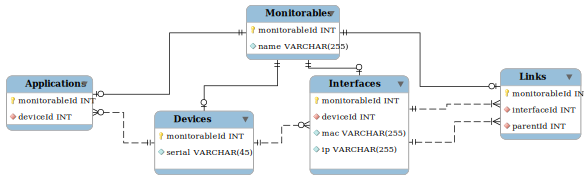
\includegraphics[width=0.9\textwidth]{contrib-asteroid-model}
		\caption{Exemple de schéma descriptif du réseau local domestique}\label{fig:contrib:asteroid:theorie:model}
	\end{figure}
\end{example}

La différence entre une donnée stable et une donnée statique est qu'il est intéressant de surveiller la modification d'une donnée (par des mécanismes tels que les \textit{triggers}) et en former un flux, qui peut être potentiellement archivé.

\textbf{Remarque} : Les clés artificielles ont une grande importance dans le cadre des applications d'observation. En effet, du fait du caractère incomplet de l'observation\footnote{soit parce que la donnée n'est pas parvenue au système, soit il n'existe pas de moyen technique pour y accéder}, il est possible d'obtenir des informations sur un équipement sans avoir pu obtenir son numéro de série. Des moyens alternatifs d'identification doivent être mis en place. Les clés artificielles permettent de tisser les relations entre les instances en ayant des données partielles. Toutefois, des vérifications d'intégrités sont nécessaires pour garder un modèle cohérent. Nous détaillons des cas applicatifs de ce problème dans nos expérimentations au chapitre~\ref{chap:valid:domvision}.

\subsubsection{Les historiques}
Supposons qu'une donnée \textit{volatile} est produite dans le flux $S$. Son historique est matérialisé par la relation temporelle $S[\infty]$. Il est nécessaire de faire persister la liste des historiques archivés. Nous modélisons cela par la création de l'association \textit{HasVolatile} donnant à partir d'un objet \textit{monitorable} et d'un \textit{volatile}, la relation contenant son historique.

D'un point de vue du schéma physique, les SGBD supportent rarement l'implémentation d'une relation dans un attribut. Pour contourner ce problème, nous créons une relation \textit{Pointers} indiquant un nom de relation historique et un attribut contenant la donnée \textit{volatile}. Ainsi, l'association \textit{HasVolatile} fournit un identifiant de pointeur au couple (\textit{monitorable, volatile}) comme montré dans la figure~\ref{fig:contrib:asteroid:theorie:volatile}.

\begin{figure}[ht]
    \centering
    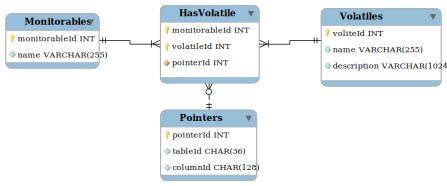
\includegraphics[width=0.8\textwidth]{contrib-asteroid-historians}
    \caption{Représentation physique de l'enregistrement des historiques}\label{fig:contrib:asteroid:theorie:volatile}
\end{figure}

\begin{example}
	Lors de l'enregistrement d'un historique de \textit{status} concernant un équipement par exemple, il est nécessaire d'insérer un n-uplet dans la relation \textit{Pointers}, qui permet de déclarer l'historique. Un autre est inséré dans \textit{HasVolatile} pour chaque \textit{monitorable} rencontré dans l'historique. Si la donnée \textit{status} n'avait pas été déclarée, il est nécessaire de le faire en insérant un n-uplet dans la relation \textit{Volatiles}.
	
	De façon similaire, les relevés de charges processeurs \textit{cpu} peuvent être attachés à un équipement ou à une application. Alors que les relevés de débits n'ont de sens que sur les interfaces (ou les liens suivant la modélisation voulue par l'utilisateur).
\end{example}

Il est intéressant de voir que puisque les données temps-réelles ont tendances à être de forte densité, il n'est peut-être pas possible de garantir une fraicheur des données au niveau du support de persistance pour les historiques.

\subsection{Représentation d'une relation persistante dans Astral}\label{sec:contrib:asteroid:theorie:astral}
Les relations issues d'un SGBD relationnel sont manipulables dans Astral du fait de leurs fondations théoriques similaires. Ainsi, une relation d'un système relationnel change au cours du temps, elle devient assimilable à une relation temporelle. Deux différences majeures subsistent : l'ordre des données et le mode d'interrogation.
\subsubsection{L'ordre d'une relation}
En SGBD, l'ordre n'importe pas jusqu'au moment de l'envoi des données à un utilisateur qui utilise le mot clé \textit{ORDER BY}. Le système peut en profiter pour modifier l'ordre lors d'opérations de jointures par exemple. Il est important de garder la même notion d'ordre au long de la requête continue. L'identifiant physique de la relation temporelle induite est par défaut la clé primaire de la relation persistante. Ainsi, nous gardons le même identifiant, et l'ordre est conservé lors des opérations.

\subsubsection{Le mode d'interrogation}
Afin d'être capable de représenter une relation temporelle dans \textit{Astronef}, il est nécessaire de pouvoir surveiller les changements effectués dans la relation persistante. Ceci peut toutefois être coûteux ou impossible suivant les moyens techniques disponibles dans le SGBD manipulé. Ainsi, pour être capable de représenter la relation telle que nous l'obtenons dans Astronef par la suite, nous utilisons un opérateur de manipulation du temps. Ce qui nous permet d'obtenir, comme indiqué dans la section~\ref{sec:contrib:astral:manipulation}, une mise à jour effective, périodique, à la demande ou inexistante.

Nous avons vu comment le SGBD peut être utilisé pour aider à la gestion de données d'observation. Nous avons aussi présenté comment représenter les relations persistantes dans Astral. Nous détaillons maintenant l'extension d'Astronef pour pouvoir manipuler le SGBD grâce à Astral.
